\documentclass[xodstep]{wnspt}

\author   {XYZ}
\nralbumu {77071} 
\kierunek {Informatyka}
\specjalnosc {Tworzenie gier komputerowych}

\date     {2024}
\miejsce {Cz\k{e}stochowa}
%\instytut {Zak\l{}adzie Informatyki Stosowanej}
\opiekun  {dr hab. Andrzej Zbrzezny}

\usepackage{amsmath}
\usepackage{amsfonts}
\usepackage{amsthm}
\usepackage{amssymb}
\usepackage[T1]{fontenc}
\usepackage[utf8]{inputenc}
\usepackage[polish]{babel}
\usepackage{polski}
\usepackage{colortbl}
\usepackage{hyperref}
\usepackage{url}
\usepackage{setspace}
\usepackage{indentfirst}
\usepackage{listingsutf8}
\usepackage{beramono}
\usepackage[section]{placeins}
\usepackage{csquotes}
\usepackage{carlito} % Dodanie czcionki Carlito
\usepackage[%backend=biber,refsegment=section,defernumbers=true,]{biblatex}


\lstset{ %
language=c++,                  % choose the language of the code
basicstyle=\ttfamily,           % the fonts that are used for the code
numbers=left,                   % where to put the line-numbers
numberstyle=\footnotesize,      % the size of the fonts that are used for the line-numbers
stepnumber=1,                   % the step between two line-numbers. If it's 1 each line will be
numbersep=5pt,                  % how far the line-numbers are from the code
showspaces=false,               % show spaces adding particular underscores
showstringspaces=false,         % underline spaces within strings
showtabs=false,                 % show tabs within strings adding particular underscores
frame=single,                   % adds a frame around the code
tabsize=4,                      % sets default tabsize to 2 spaces
captionpos=b,                   % sets the caption-position to bottom
breaklines=true,                % sets automatic line breaking
breakatwhitespace=false,        % sets if automatic breaks should only happen at whitespace
escapeinside={\%*}{*)}          % if you want to add a comment within your code
}

\newcommand{\R}{mathbb{R}}

\renewcommand{\lstlistlistingname}{Spis listingów}
\renewcommand{\lstlistingname}{Listing}

\newtheorem{lemat}{Lemat}
\newtheorem{twierdzenie}{Twierdzenie}

\title{\begin{LARGE}Optymalizacja interfejsów użytkownika w grach wirtualnej rzeczywistości: Perspektywa programisty i projektanta UX/UI
\\{~}
Optimizing user interfaces in virtual reality games: A developer and UX/UI designer's perspective
\end{LARGE}}

\frenchspacing
\begin{document}
\begin{abstract}
Celem pracy dyplomowej było opisanie i opracowanie projektu interfejsu użytkownika
Dokonano analizy konkurencji, zaprojektowano 
Przebudowano gotowe systemy
Wdrożony system został przetestowany potwierdzając poprawne działanie.


Opisano również dalsze możliwości rozwoju gry.
\end{abstract}

\keywords{Virtual Reality,  User Interaction, Immersion, Vr Interface Design, Human-Centered Design}
\maketitle

\onehalfspacing

\introduction

Rzeczywistość wirtualna dynamicznie się rozwija i znajduje wykorzystanie w coraz szerszym zakresie dziedzin, takich jak edukacja, architektura, medycyna czy budownictwo. VR umożliwia użytkownikom przeżywanie doświadczeń niemożliwych lub (problematycznych?) do osiągnięcia w prawdziwym życiu. 
Jednym z kluczowych elementów wpływających na doświadczenia użytkowników jest odpowiednio zaprojektowany interfejs użytkownika (UI). Interfejsy te umożliwiają nie tylko łatwą i intuicyjną interakcję z produktem, ale są również wyjątkowo istotne w zapewnieniu odbiorcom komfortu i nieprzerwanej imersji, która jest kluczowym elementem VR. Projektowanie interfejsu użytkownika w rzeczywistości wirtualnej musi uwzględniać charakterystyczne cechy tej technologii, takie jak przestrzeń trójwymiarowa, specyficzne sposoby interakcji oraz różnorodne potrzeby użytkowników.

Celem niniejszej pracy jest wybór oraz zaprojektowanie najbardziej optymalnego interfejsu użytkownika, który będzie charakteryzować się uniwersalnym zastosowaniem w różnych środowiskach VR. Praca ma na celu zidentyfikowanie najważniejszych elementów interfejsów użytkownika, które zapewnią największy komfort i nieprzerwaną immersję oraz zaprojektowanie gotowego rozwiązania.
W ramach pracy zostaną zaprezentowane rożne podejścia do interakcji w wirtualnej rzeczywistości które następnie zostaną dostosowane do różnorodnych potrzeb użytkowników oraz uwzględnią ograniczenia motoryczne, sensoryczne czy poznawcze. Proces ten pozwoli na wybór najbardziej efektywnego i wszechstronnego rozwiązania, które można zastosować w rożnych aplikacjach i grach VR

Wybór tematu wynika z rosnącego zapotrzebowania na rozwój interfejsów użytkownika w VR, szczególnie w kontekście coraz to nowszych zastosowań tej technologi, takich jak edukacja medycyna czy budownictwo. Na rynku istnieje duża luka, jeśli chodzi o projektowanie zorientowane na człowieka (HCD) uniwersalnych interfejsów użytkownika, które byłyby zarówno dostępne jak i wygodne dla osób z rożnymi ograniczeniami. Po doświadczeniach z z różnymi grami i aplikacjami VR, zauważyłam, że wiele z nich nie spełnia oczekiwań w zakresie dostosowania do potrzeb osób z problemami motorycznymi lub sensorycznymi. Takie doświadczenia skłoniły mnie do podjęcia próby rozwiązania tych problemów i stworzenia rozwiązania, które zapewni komfort i dostępność dla wszystkich użytkowników.

Podczas realizowania tego projektu napotkam szereg różnych wyzwań związanych z pełnieniem różnych rol w procesie tworzenia interfejsu użytkownika w rzeczywistości wirtualnej. Pierwszym z nich będzie konieczność dostosowania interfejsu do trójwymiarowej przestrzeni VR, co wiąże się z nowymi zasadami ergonomii i interakcji. Jako osoba odpowiedzialna za cały projekt, będę samodzielnie pełniła funkcje UX Rasearchera, UX/UI Designera, programisty oraz testera. Jako UX Researcher, będę miała za zadanie przeprowadzić badania użytkowników w celu identyfikacji potrzeb preferencji i punktów bólu w kontekście VR, a następnie zaprojektować interfejs dostosowany do rożnych grup odbiorców. Rola UX/UI designera wiąże się z zaprojektowaniem funkcjonalnych i estetycznych elementów interfejsu spójnych z wymaganiami rzeczywistości wirtualnej. Jako programistka będę odpowiedzialna za implementacje interfejsu i zapewnienie optymalizacji działania. Dodatkowo, jako tester, będę przeprowadzała testy, identyfikowała punkty bólu i problemy a następnie wprowadzała poprawki na podstawie uzyskanych wyników.

Praca została podzielona na pięć głównych rozdziałów. Rozdział pierwszy wprowadza do ogólnych zasad projektowania interfejsów, koncentrując się na podejściu projektowym, który kładzie nacisk na użytkownika. Omówione zostaną kluczowe zasady UX/UI, takie jak ergonomia, intuicyjność, przejrzystość i użyteczność interfejsów. Rozdział drugi będzie skupiał się na porównaniu interfejsów wykorzystywanych na tradycyjnych platformach z tymi występującymi w wirtualnej rzeczywistości. Zawiera szczegółową analizę wpływu trójwymiarowej przestrzeni VR na projektowanie interakcji oraz przedstawia wyzwania związane z adaptacją zasad UX/UI do specyfiki tej technologii. Rozdział trzeci zawiera proces projektowania interfejsu VR w narzędziach takich jak Figma jednocześnie omawiając proces tworzenia interaktywnych elementów i testowanie rożnych układów i metod interakcji. W czwartym rozdziale uwzględniono implementacje zaprojektowanego rozwiązania w środowisku VR.
% (to jeszcze wyjdzie w trakcie pisania pracy ale planowałam aby w tym rozdziale był również szczegółowy opis wybranych metod interakcji np  ekran 180 stopni albo otwierana książka razem z analizą pod kątem trudności w implementacji szybkością realizacji i wygody użytkowania)
W piątym rozdziale zostanie wybrana odpowiednia metoda badawcza, najlepiej dopasowana do charakterystyki projektu oraz dostępnych zasobów. Celem tej części pracy jest zebranie informacji od użytkowników dotyczących użyteczności zaprojektowanego interfejsu. Po dokonaniu wyboru metody badawczej, przeprowadzone zostaną testy użytkowników, które pozwolą na ocenę intuicyjności, efektywności i komfortu interakcji z gotowym produktem. Po zakończeniu testów, uzyskane wyniki zostaną poddane analizie, co umożliwi dalszą optymalizację interfejsu. 
%(tu nie wiem czy nie dodać rozdziału albo podrozdziału do sekcji badan z wprowadzeniem poprawek do punktow bólu wykrytych podczas badań)
W zakończeniu pracy podsumowane zostaną główne wnioski oraz zaproponowane kierunki dalszych badań i rozwoju interfejsów VR, a także rozważone możliwości komercjalizacji opracowanych rozwiązań.

%Mam problem z klawiaturą  - ó 

\chapter{Wprowadzenie do tematyki pracy, wykorzystane narzędzia}
%Ten rozdział mi nie gra jakoś, narzędzia są okej ale reszta mi nie pasuje
\section{Technologia VR}
Technologia rzeczywistości wirtualnej polega na tworzeniu w pełni sztucznego otoczenia, które wywołuje poczucie przebywania w zupełnie innym miejscu lub świecie. Dzięki specjalistycznym urządzeniom, takim jak gogle czy kontrolery ruchu, możliwe staje się obserwowanie i oddziaływanie na generowane wirtualnie obiekty w czasie rzeczywistym. Rozwiązania z zakresu VR wykorzystują zaawansowane techniki renderowania grafiki, precyzyjnie śledzą ruch głowy i dłoni, a także uwzględniają dźwięk przestrzenny, co pozwala na osiągnięcie wysokiego stopnia imersji. Technologia ta znajduje zastosowanie nie tylko w obszarze gier i rozrywki, lecz również w szkoleniach branżowych, symulacjach medycznych \ref{vr_example} i architektonicznych oraz w przemyśle, gdzie służy do prototypowania i prezentacji projektów. Wirtualna rzeczywistość sprzyja ograniczaniu kosztów wdrożeń oraz podnoszeniu efektywności procesów nauki i projektowania, ponieważ umożliwia wielokrotne testowanie różnych scenariuszy w ściśle kontrolowanym środowisku.

\begin{figure}[!htb]
    \centering
    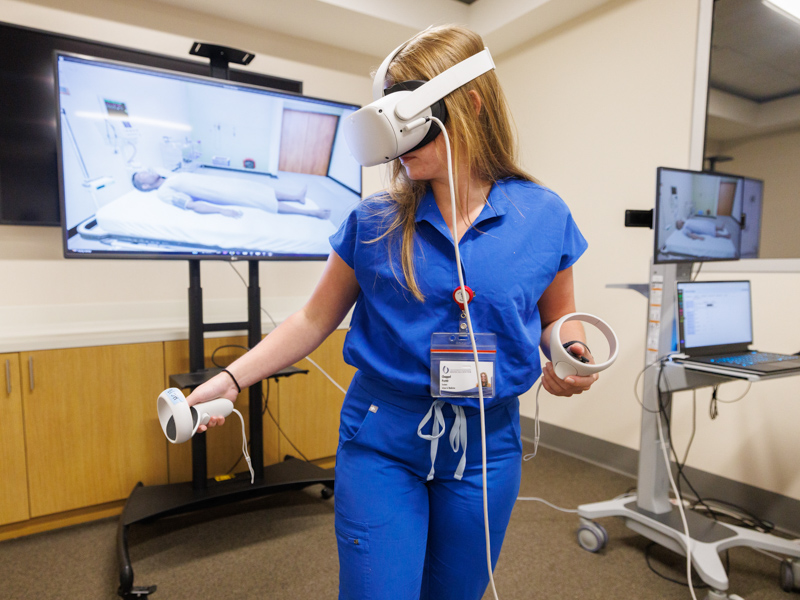
\includegraphics[width=0.8\textwidth]{images/vr_example.jpg}
    \caption{Symulator medyczny służący do szkolenia lekarzy}
    \label{vr_example}
\end{figure}\textbf{}


 \section{Znaczenie UX w procesie projektowania}
 
 W sytuacji, gdy użytkownik napotyka trudności w interakcji z przedmiotem, takim jak drzwi, i nie wie, jak wykonać określoną czynność (np. otworzyć drzwi), problemem nie jest sam użytkownik, lecz projekt produktu(Norman, 2013).



\section {Narzędzia i środowisko pracy}


 projektowania tej pracy był wybór odpowiednich narzędzi umożliwiających prototypownie, implementację oraz testowanie interfejsu w środowisku VR. Wybór używanej technologii jest kluczowy, aby zapewnić wysoką jakość doświadczeń użytkownika oraz zachować efektywność samego procesu projektowania.

\subsection{Figma}
Figma to podstawowe narzędzie służące do projektowania interfejsów użytkownika, jednocześnie umożliwia tworzenie interaktywnych klikalnych prototypów aplikacji. Jest to aktualnie jedno z najbardziej popularnych i bezpłatnych narzędzi w branży UX/UI. W projekcie Figma zostanie wykorzystana do stworzenia wstępnych projektów i prototypów interfejsów, a następnie do przetestowania rożnych układów elementów interfejsu. 
%(tu będzie dokumentacja figmy)
\subsection{Unity}
\textit{Unity} to jeden z najpopularniejszych wieloplatformowych silników do tworzenia gier wideo oraz interaktywnych aplikacji. Umożliwia zaawansowaną obsługę grafiki i fizyki, a w samym edytorze udostępniono rozbudowany zestaw narzędzi do projektowania scen, animacji i efektów graficznych \ref{unity_engine_example}. Proces programowania odbywa się przy użyciu języka \textit{C\#}.

W Unity dodano również wsparcie dla wirtualnej oraz rozszerzonej rzeczywistości, co przekłada się na szerokie zastosowanie tej technologii w szkoleniach, symulacjach czy działaniach marketingowych. Oprócz możliwości tworzenia zaawansowanych pod względem wizualnym scen, istotna jest też opcja łatwej integracji gotowych wtyczek obsługujących urządzenia AR i VR od różnych producentów. Rozbudowany system oświetlenia oraz post-processingu zapewnia szeroki wachlarz opcji i umożliwia dostosowanie grafiki pod dedykowane urządzenia, dzięki czemu można uzyskać zadowalającą jakość i odpowiednią optymalizację na urządzenia mobilne oraz wysoce realistyczną grafikę na komputerach osobistych.

\begin{figure}[!htb]
    \centering
    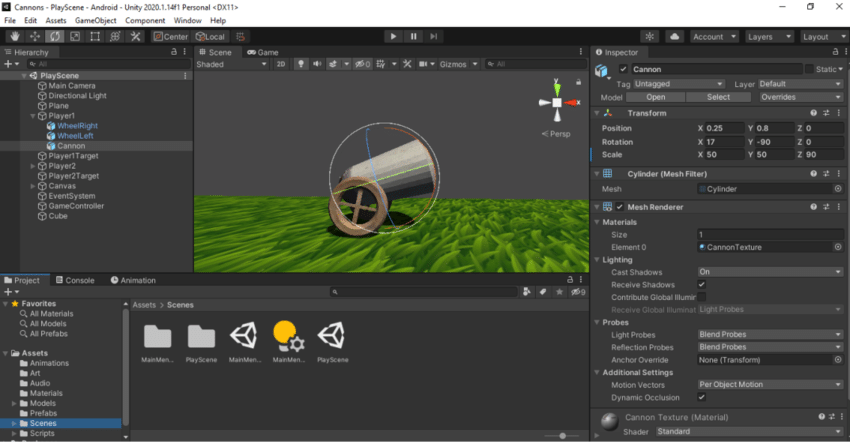
\includegraphics[width=0.8\textwidth]{images/unity.png}
    \caption{Przykładowy wygląd edytora Unity}
    \label{unity_engine_example}
\end{figure}

Regularne aktualizacje silnika rozszerzają jego funkcjonalność i dodają nowe rozwiązania, takie jak obsługa ray tracingu, DLSS oraz nowe narzędzia. Stały rozwój sprawia, że Unity zachowuje elastyczność w obliczu zmieniających się potrzeb rynku, a jego wszechstronność umożliwia realizację nawet najbardziej rozbudowanych koncepcji interaktywnych.

Społeczność skupiona wokół tego silnika udostępnia liczne materiały edukacyjne w postaci kursów i filmów, co znacząco obniża poziom wejścia, przyspiesza naukę oraz ułatwia rozwiązywanie ewentualnych problemów technicznych. Dokumentacja silnika jest regularnie rozwijana, a oficjalny sklep \textit{Asset Store} zapewnia dostęp do bardzo dużej ilości bezpłatnych oraz płatnych pakietów, obejmujących zasoby takie jak modele, tekstury i dźwięki oraz dodatkowe użyteczne narzędzia wraz z całymi gotowymi systemami ułatwiającymi stworzenie projektu i pozwalającymi ograniczyć koszty produkcji.


\subsection{Gogle VR}
Gogle VR to urządzenia, które całkowicie zasłaniają pole widzenia i wyświetlają przez użytkownikiem dwa identyczne, ale nieco przesunięte od siebie obrazy, które nałożone na siebie przez mózg dają wrażenie głębi. Wewnątrz gogli umieszczone są specjalne czujniki takie jak żyroskop, kamery i inne śledzące położenie i ruch głowy w przestrzeni. Dzięki temu użytkownik obracając głową faktycznie rozgląda się w przestrzeni wirtualnej obracając kamerą gracza.

Oprócz gogli istotne są również specjalne kontrolery zakładane na dłonie. Dzięki nim możliwa jest interakcja z wirtualnym otoczeniem, a specjalne czujniki i przyciski wykrywają pozycje palców i pozwalają określić, czy gracz w tej chwili próbuje złapać przedmiot. Całość wraz z systemem śledzenia pozycji dłoni pozwala dowolnie sięgać w różnych kierunkach, co pozwala mieć wpływ na obiekty w aplikacji. Gracz może na przykład chwycić przedmiot i rzucić nim, co pozwoli wywołać kolejne symulacje w fizyce.

Oprócz tego istnieje wiele różnych dodatków rozszerzających możliwości wirtualnej rzeczywistości, jak specjalne kombinezony monitorujących ruch oraz umożliwiających odczuwanie na skórze poprzez elektrostymulację nerwów i mięśni lub kapsuły, w których użytkownik ma możliwość skakania oraz poruszania się w dowolny sposób bez ryzyka, że uszkodzi coś w pokoju.

\subsection{Google Forms i inne narzędzia do analizy UX/UI}








%Tworzenie interfejsów użytkownika w środowisku wirtualnej rzeczywistości wiąże się z wieloma trudnościami, które nie występują w tradycyjnych aplikacjach. Ze względu na trójwymiarowy wymiar wirtualnej rzeczywistości konieczne będzie zastosowanie nowych zasad ergonomii, ktore umożliwią użytkownikom komfortową, intuicyjną oraz płynną interakcję z produktem. Przy projektowaniu należy wziąć pod uwagę takie aspekty jak ograniczenia technologiczne i sensoryczne jak np. pole widzenia czy ograniczenia motoryczne użytkowników. 

%\section{Ogólne zasady projektowania interfejsów użytkownika}
\chapter{Podstawowe Zasady UX/UI designu}

\section{Wprowadzenie do UX Designu}

 UX design, czyli projektowanie doświadczeń użytkownika, to proces tworzenia zapewniający pozytywne doświadczenia użytkownikom poprzez optymalizacje interakcji z daną stroną, systemem czy produktem. Początkowo zagadnienie to było kojarzone głównie z projektowaniem stron internetowych i aplikacji, jednak współczesne podejście znajduje zastosowanie w każdej dziedzinie. Obecnie UX design obejmuje projektowanie przeróżnych produktów, od stron internetowych po urządzenia codziennego użytku jak urządzenia AGD, samochody czy nawet meble. Aktualnie UX odnosi się nie tylko do wirtualnych interfejsów ale także do interakcji ze zwykłymi przedmiotami z którymi styczność mamy wszyscy.


\section{Podstawowe Zasady UX/UI}

Autorzy rożnych książek wyróżniają szereg fundamentalnych zasad UX designu, które pomagają w tworzeniu bardziej efektywnych, intuicyjnych i przyjemnych doświadczeń użytkowników.
Wśród kluczowych zasad projektowania UX/UI wyróżnia się:


\subsection{Ergonomia i Prostota}
Produkt powinien być projektowany tak, by był wygodny i łatwy w użyciu. Dobre projektowanie UX uwzględnia nie tylko interakcje użytkownika z urządzeniem, ale również sposób, w jaki przetwarza on informacje wyświetlane na ekranie. Produkt powinien być dostosowany do naturalnych zdolności i ograniczeń użytkownikow zapewniając im płynne i efektywne osiąganie zamierzonych celow.(Don Norman, 2013).

Zasada Prostoty oznacza elimniowanie zbędnych elementow i skomplikowanych funkcji, ktore mogą rozpraszać uwage odbiorcy lub sprawiać że produkt staje sie trudny w obsłudze. Koncentruje sie głownie na tym z czego użytkownik będzie rzeczywiscie korzystał Prostota podczas projektowania interfejsow polega na tym, ze wszystkie funkcjonalności są dostępne dla użytkownika w oczywisty i jak najprostszy sposob. Dązenie do prostoty w projekcie jest istotne ponieważ pomaga zapobiec przeciązeniu poznawczemu ktore może wystąpić gdy system jest zbyt skomplikowany. 


\subsection{Widoczność i Intuicyjność}

Dobrze zaprojektowany pod względem widoczności interfejs powinien sprawiać by użytkownik był w stanie łatwo dostrzec dostępne opcje funkcje bez konieczności szukania. Elementy powinny by umieszczone w miejscach w których naturalnie się ich spodziewają. Pozwala to na szybkie zrozumienie sposobu poruszania się w systemie. Zasada ta uwzględnia również umiejscowienie mniej istotnych elementów, takie jak ustawienia lub dodatkowe funkcje. Nie muszą one być widoczne na pierwszy rzut oka, ważne jest aby były one nadal łatwe do zlokalizowania w razie potrzeby. Don Norman

Intuicyjność oznacza, że interfejs powinien być zaprojektowany w taki sposób aby użytkownik mógł naturalnie zrozumieć jego działanie opierając się na swoich wcześniejszych doświadczeniach i oczekiwaniach. Elementy powinny być widoczne i łatwe do zlokalizowania oraz reagować zgodnie z jego przyzwyczajeniami. Sposób poruszania się po systemie powinien być dla nich oczywisty. Steve Krug

\subsection{Dostępność i Informacja zwrotna}
Zasada dostępności jest bardzo ważna, aby zapewnić by wszyscy użytkownicy, niezależnie zdolności fizycznych, sensorycznych czy poznawczych  byli w stanie korzystać z aplikacji. Treść interfejsu powinna być jasna i zrozumiała a teksty powinny być odpowiednio widoczne  z dobrym kontrastem miedzy tłem a literami. Elementy interaktywne takie jak przyciski, suwaki powinny być łatwe do znalezienia i i użyteczne. Powinien również  oferować użytkownikom dostosowania jego wyglądu , na przykład zmianę rozmiaru tekstu lub kontrastu. Designing Interfaces Jenifer Tidwell

Jest to reakcja systemu na działania, które wykonuje użytkownik pozwalając mu na kontrolowanie swoich interakcji z systemem i ich efektów w czasie rzeczywistym. Dobre projektowanie interfejsu zapewnia, że każda interakcja użytkownika, taka jak kliknięcie przycisku czy zmiana ustawienia, zostanie natychmiastowo potwierdzona odpowiednią reakcją systemu. Reakcja może przybierać różne formy, jak wizualna czy dźwiękowa.(Saffer, 2006)


\section{Róznice w projektowaniu interfejsu VR}
Chociaż większość podstawowych zasad UX designu jest uznawana jako uniwersalana to projektowanie interfejsu użytkownika w oparciu o nie wymaga od projektanta innego podejścia. Wynika to z odmienności systemu VR od innych technologii, takich jak aplikacje mobilne, aplikacje desktopowe czy strony internetowe, gdzie wszystkie interakcje z systemem odbywają się za pomocą myszki, klawiatury, ekranów dotykowych ewentualnie czytników ekranów. Tworzenie interfejsów użytkownika w środowisku wirtualnej rzeczywistości wiąże się z wieloma trudnościami, które nie występują w tradycyjnych aplikacjach. W projekcie konieczne będzie dostosowanie zasad tak, aby umożliwić użytkownikom komfortową, intuicyjną oraz płynną interakcję z produktem. Przy projektowaniu należy wziąć pod uwagę takie aspekty jak ograniczenia technologiczne i sensoryczne jak np. pole widzenia czy ograniczenia motoryczne użytkowników. 

Pierwszą fundamentalną różnicą między tradycyjnym wykorzystaniem zasad UX designu jest \textbf{Nawigacja}. W przypadku stron internetowych i aplikacji przemieszczanie się po produkcie odbywa się za pomocą klikania ikon, przewijania, ruchów myszką czy naciskania odpowiednich przycisków na klawiaturze. W wirtualnej rzeczywistości nawigowanie polega w głównej mierze na ruchach użytkownika szczególnie w przypadku bardziej zaawansowanych urządzeń takich jak  Pico 4 Ultra Enterprise, które nie wymagają dodatkowych urządzeń a korzystanie z nich odbywa się bezprzewodowo.(https://vr-expert.com/pl/samodzielne-vr/). Przemieszczanie po systemie odbywa się za pomocą śledzenia ruchow głową i ciała za pomocą kontrolerów ruchów. Często stosowane są również abstrakcyjne metody przemieszczania się jak np, teleportacja do innego miejsca oddalonego w przestrzeni co umożliwia eksplorowanie większych środowisk VR (Jennifer Whyte Dragana Nikolić - Virtual Reality and the Built Environment-Routledge (2018). Sam interfejs jest też inaczej umieszczony w przestrzeni. Tradycyjnie osadzone są w przestrzeni ekranu. W wirtualnej rzeczywistości interfejsy są umieszczone w przestrzeni  świata. Elementy mogą lewitować przed użytkownikiem lub częscią być częścią otoczenia. (Jonathan Linowes - Unity Virtual Reality Projects - Second Edition)
Następna równie ważna różnica to \textbf{Interakcja w przestrzeni 3D}. W tradycyjnych interfejsach  użytkownik wchodzi w interakcje z płaskimi, dwuwymiarowymi elementami na ekranie. W VR interakcje odbywają się w przestrzeni trójwymiarowej a użytkownik może dowolnie manipulować  obiektami tak jakby były on prawdziwe. Umożliwia chwytanie obracanie i przesuwanie element za pomocą rąk oraz interakcje które wymagają pełnego zaangażowania ciała użytkownika jak np. schylanie czy kucanie co wpływa pozytywnie na immersje i realizm doświadczenia.
Pozwala również na odejście od zgodności z rzeczywistością(nie wiem czy  to dobry synonim dla realizmu) i umożliwia działania niemożliwe w prawdziwym świecie jak przemieszczanie przedmiotów oddalonych w dużej odległości czy teleportacja. (Virtual, Augmented and Mixed Reality)
\textbf{Projektowanie interakcji} w wirtualnej rzeczywistości wymaga naśladowania w jaki sposob użytkownicy wchodzą w interakcje z przedmiotami i otoczeniem w prawdziwym świecie. Gesty i ruchy powinny być realistycznie odwzorowane a odpowiedz systemu natychmiastowa. Tradycyjne interakcje są bardziej pośrednie, gdy użytkownik chce wykonać jakieś działanie musi poruszyć myszką aby na ekranie kliknąć w pożądaną ikonę. W VR możliwe jest fizyczne "podniesienie" przedmiotu lub otwarcie drzwi.(Multimedia and Virtual Reality - Alistair Sutcliffe)    
W grach komputerowych czy aplikacjach rzadko zdarza się aby użytkownik odczuwał dyskomfort fizyczny, jedynym czynnikiem mogącym zakłócić poczucie komfortu jest natknięcie się na elementy wywołujące fobie, takie jak arachnofobia czy klaustrofobia. VR oferuje o wiele większą immersje niż gry na komputer i pozwalają użytkownikowi na pełne zanurzenie się w rozgrywkę ale torzenie treści do tego środowiska wymaga zachowania większej ostrożności aby uniknąć efektow ubocznych. Jednym z nich jest choroba symulatorowa (VR sickness).

\begin{figure}[!htb]
    \centering
    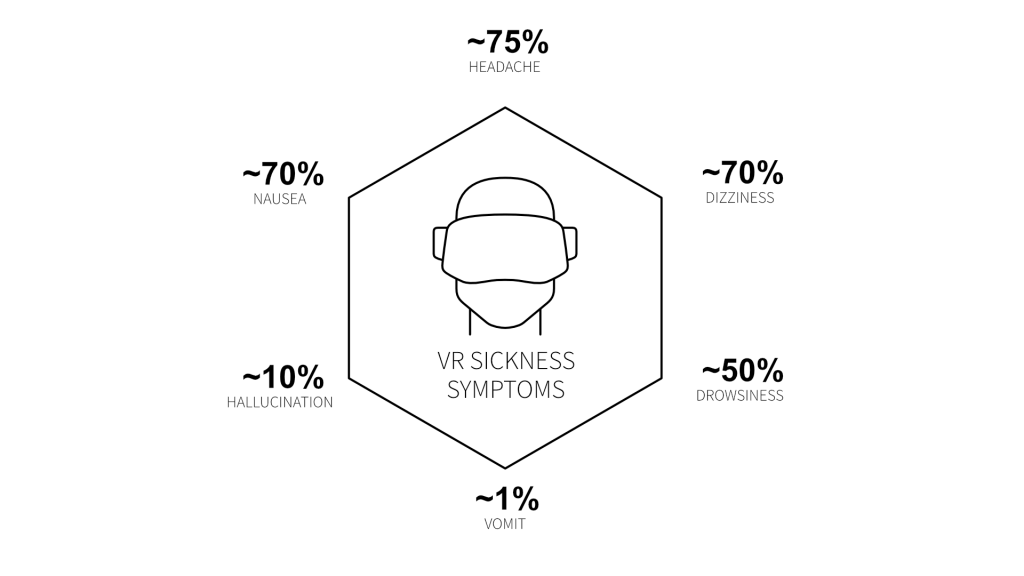
\includegraphics[width=0.8\textwidth]{images/VRSICK.png}
    \caption{Przykładowy wygląd edytora Unity}
    \label{unity_engine_example}
\end{figure}

Choroba ta jest bardzo powszechna wśród osób korzystających z wirtualnej rzeczywistości. Objawia się najczęściej mdłościami, zawrotami głowy czy ogólna dezorientacją. \textbf{}{Komfort użytkownika i jego adaptacja fizyczna} jest więc kluczowymi aspektami projektowania interfejsów użytkownika. (3D user Interfaces Theory and Practice)

Interakcje z produktami na komputery i telefony opierają się głownie na płaskich bodźcach wizualnych i dźwiękowych. Ogranicza to poziom zaangażowania odbiorcy i wpływa na mniej intensywne doświadczenia. Natomiast wirtualne środowisko może angażować nie tylko słuch i wzrok ale również dotyk poprzez kontrolery z haptyczna czy wibracje. Wirtualna rzeczywistość angażuje różne \textbf{zmysły}, aby maksymalnie zwiększyć zanurzenie użytkownika w cyfrowym świecie i zapewnić mu jak najlepsze doznania
 
Podane różnice dowodzą, że projektowanie interfejsu dla VR wymaga zupełnie innego podejścia niż w przypadku tradycyjnych gier i aplikacji. 


\section{Zasady  projektowania UX/UI w kontekście aplikacji VR}

W kontekście VR projektowanie interfejsów staje się szczególnie problematyczne ze względu na konieczność osiągnięcia równowagi między imersją w wirtualnej rzeczywistości a zapewnieniem intuicyjnej interakcji oraz komfortu użytkowania, dlatego istotne jest zastosowanie sprawdzonych zasad UX/UI dostosowanych pod to środowisko



\textbf{
SZANOWNY PANIE PROFESORZE- ZE WZGLĘDU NA PROBLEM Z LITERĄ ó wszystkie słowa wykorzystujące te literę będę pisała z o ponieważ jestem w stanie to potem szybko zamienić 
DZIĘKUJE ZA ZROZUMIENIE. 
Szukałam rozwiązania w internecie ale nikt nie miał podobnego problemu więc jest to najprawdopodobniej wina klawiatury}
\chapter{Projektowanie interfejsu VR}


\section{Analiza rozwiązań istniejących już na rynku}
Projektowanie interfejsu do VR może odbywać się na kilka różnych sposobów różniących się od siebie sposobem integracji z wirtualnym środowiskiem i tym jak prezentowane są istotne informacje. Aby odpowiednio przygotować się do projektowania, należy zapoznać się z najczęściej stosowanymi rozwiązaniami w istniejącymi już na rynku produktach. Należy zrozumieć co twórcy gier i symulatorów uznali za ważniejsze, pełną immersje czy raczej stawiali na tradycyjne menu i lewitujące w przestrzeni wirtualnej panele. W pierwszej kolejności warto jednak poznać kilka podstawowych rodzajów interfejsow i czym sie charakteryzują. Pozwoli to na lepsze zrozumienie jak i kiedy są one wykorzystywane. Na potrzeby analizy zastosowano podział interfejsów na cztery najczęściej stosowane rodzaje. Interfejs jako część świata gry, Klasyczny panel menu (Non-diegetic UI), Interfejs panelowy w środowisku VR (Spatial UI) oraz HUD (Head-Up Display.
Pierwszy rodzaj polega na wpleceniu interfejsu w elementy już istniejące w świecie wirtualnym, użytkownik żeby go zobaczyć musi fizycznie skierować głowę na dany element. Drugi z kolei wykorzystuje tradycyjny panel menu, ktory możemy spotkać na stronach internetowych czy w grach na komputer. Elementy interfejsu nie są częścią otoczenia a sam panel jest nakładką na widok użytkownika. Kolejne podejście to interfejs panelowy ale umieszczony w środowisku wirtualnym. Typ ten charakteryzuje się unoszącym się w powietrzu menu, które może być sterowane za pomocą kontrolera lub ruchami rąk. Ostatni typ to HUD, rodzaj stosowany często w tradycyjnych grach. Najważniejsze informacje są "przyklejone" do widoku gracza, pozostając cały czas w jego polu widzenia niezależnie od miejsca w którym znajduje się użytkownik w wirtualnym otoczeniu.

\subsection{Half-Life: Alyx}

Pierwszy rodzaj polega na wpleceniu interfejsu w elementy już istniejące w świecie wirtualnym a użytkownik żeby go zobaczyć musi fizycznie skierować głowe na dany element. Może to być wyświetlacz kokpitu  czy ekran Monitora
No Man’s Sky VR, Interfejs panelowy w środowisku VR (Spatial UI)


(Jonathan Linowes w Unity Virtual Reality Projects)



\subsection{Beat Saber}
Phasmophobia VR
Beat Saber

\subsection{No Man's Sky}

https://ekspert.ceneo.pl/najlepsze-gry-vr


\subsection{Symulator VR „Zaawansowane procedury medyczne”
}
"Rozwija praktyczne umiejętności studentów w zakresie segregacji medycznej, udzielania kwalifikowanej pierwszej pomocy, podstawowej pierwszej pomocy oraz ratownictwa medycznego. Posiada edytor umożliwiający wybór odpowiedniego środowiska, konfigurację pacjentów, dostępnego sprzętu i wartości referencyjnych. Dostępny jest w trybach: egzaminacyjnym lub ćwiczeniowym; jedno bądź wieloosobowym oraz w wariancie PC i VR."



\subsection{Komentarz}
Zastanawiam się czy nie skupić się głownie na symulatorach. Interfejsy w grach najczęściej są wyjątkowo dopracowane aby rozgrywka odbywała się płynnie. W przypadku symulatorów szczególnie edukacyjnych rozwiązania są rozbudowane pod względem mechanik w samej rozgrywce ale sposób przekazywania informacji jest tragiczny, Interakcje odbywają sie głownie za pomocą lasera a sam interfejs utrudnia wykonywanie czynności. Brakuje tam naśladowania jak te czynnści odbywają się w prawdziwym świecie. Przykładowo w symulatorze kryminalistyki możemy pobierać odciski buta itp ale wyciaganie przedmiotow odbywa sie nieintuicyjnie i rozpraszająco za pomocą interfejsu panelowego umieszczonego w przestrzeni. Zaprojektowanie interfejsu głownie do symulatorów będzie również bardziej logiczne bo głownym ich celem jest nauka a w przypadku gier cele mogą być rozne. Niektore chcą wystraszyc gracza a inne żeby spokojnie eksplorował stworzony świat.

https://uxdesign.cc/vr-diegetic-interfaces-dont-break-the-experience-554f210b6e46


\section{Tworzenie prototypów interfejsów użytkownika dla VR}
Aby uniknąć wielokrotnej implementacji niezliczonej ilości ilości interfejsów 
\section{Testowanie różnych układów elementów i metod interakcji}
%(kontrolery, gesty, głos).
\section{Projektowanie interaktywnych obiektów}
\subsection{obiekt fizyczny dynamiczny}
\subsection{obiekt fizyczny statyczny}
\subsection{obiekt wirtualny}
\section{Tworzenie elementów wizualnych}
%Tworzenie atrakcyjnych wizualnie i funkcjonalnych przycisków.



wstępne testy użyteczności z uzytkownikami 
Weryfikacja efektywności i intuicyjności interakcji
Iteracyjne poprawki na podstawie wyników testów

\chapter{Implementacja interfejsu w środowisku VR}

/section{Implementacja sposobu 1}
/section{Implementacja sposobu 2}
/section{Implementacja sposobu 3}
Zastosowanie wybranych metod interakcji


\summary
Założony cel tej pracy, aby 


\bibliographystyle{plain}
\printbibliography[type=book,title={Books only}]
%Cały czas mam problem z tą bibliografią. Podczas inżynierki probowałam to naprawić z doktor Lidią Stępień ale niestety nie udało nam się tego naprawić 
% spis rysunków (jeżeli jest potrzebny):
\listoffigures

% spis listingów (jeżeli jest potrzebny):
\lstlistoflistings

\end{document}
